% Source for the figure of ThreadPool (sec. 25.3): the deques of a pool of
% p = 4 threads when the caller, in the slot 0, has pushed the h = 3 tokens
% of a job of bulk(), and after two thieves have stolen one token each.
% Build: make figures (in ../build).
\documentclass[border=4pt]{standalone}
\usepackage[T1]{fontenc}
\usepackage{newpxtext,newpxmath}
\usepackage[varqu,varl,scaled=0.95]{zi4}
\usepackage{tikz}
% tikz-ads.tex: the TikZ styles shared by the figures of the memory of the
% manual, \input by each standalone figure: a cell of a vector (cell), the
% cell that an operation touches (touched), a free cell (free), a node of a
% linked structure (node), the labels of indices (index) and of variables
% (var), a pointer (ptr), and \cells and \indices to draw a row of cells.
\usetikzlibrary{arrows.meta,positioning,calc,fit,shapes.multipart}
\definecolor{adsTouched}{RGB}{214,196,236}
\definecolor{adsFree}{RGB}{236,236,236}
\tikzset{
  ads/.style={>={Stealth[length=2mm]},font=\small,
              every node/.append style={inner sep=0pt}},
  cell/.style={draw,minimum width=7mm,minimum height=7mm,
               font=\small\ttfamily,outer sep=0pt},
  touched/.style={cell,fill=adsTouched},
  free/.style={cell,fill=adsFree,text=black!45},
  node/.style={draw,rounded corners=1pt,minimum width=8mm,
               minimum height=6mm,font=\small\ttfamily},
  index/.style={font=\scriptsize\ttfamily,text=black!60},
  var/.style={font=\small\itshape},
  ptr/.style={->,thick}
}
% \cells{name}{x,y}{list}: a row of cells, the first at (x,y), named
% name-0, name-1, ...; each item is text/style, the style one of cell,
% touched and free (e.g., {a/cell,e/touched,/free})
\newcommand{\cells}[3]{%
  \foreach \v/\s [count=\i from 0] in {#3}
    \node[\s] (#1-\i) at ($(#2)+(\i*7mm,0)$) {\v};}
% \indices{name}{n}: the indices 0 .. n-1 under the cells of name
\newcommand{\indices}[2]{%
  \foreach \i in {0,...,\numexpr#2-1\relax}
    \node[index,below=1.2mm of #1-\i] {\i};}

\begin{document}
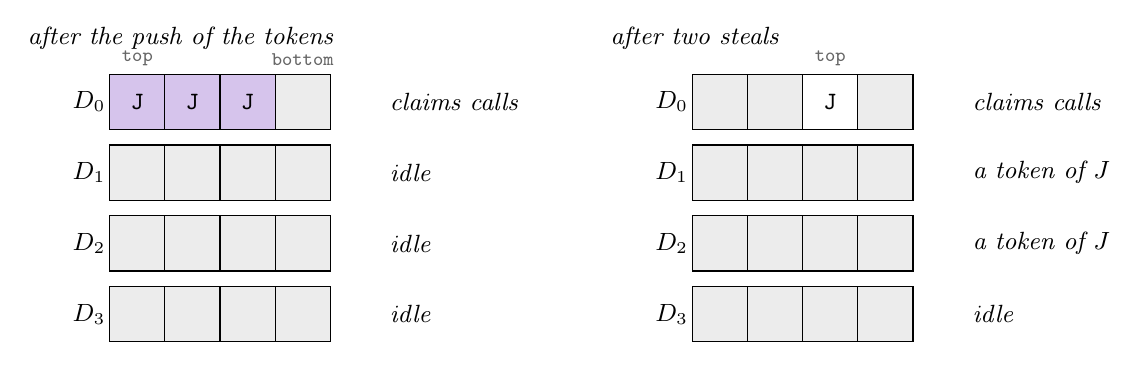
\begin{tikzpicture}[ads]
  % before the steals
  \node[var,anchor=west] at (-14mm,8mm) {after the push of the tokens};
  \foreach \s/\y in {0/0,1/-9mm,2/-18mm,3/-27mm} {
    \node[var,anchor=east] at (-4mm,\y) {$D_{\s}$};
  }
  \cells{a}{0,0}{J/touched,J/touched,J/touched,/free}
  \cells{b}{0,-9mm}{/free,/free,/free,/free}
  \cells{c}{0,-18mm}{/free,/free,/free,/free}
  \cells{d}{0,-27mm}{/free,/free,/free,/free}
  \node[index,above=1mm of a-0] {top};
  \node[index,above=1mm of a-3] {bottom};
  \node[var,anchor=west] at (32mm,0) {claims calls};
  \node[var,anchor=west] at (32mm,-9mm) {idle};
  \node[var,anchor=west] at (32mm,-18mm) {idle};
  \node[var,anchor=west] at (32mm,-27mm) {idle};
  % after two steals
  \begin{scope}[xshift=74mm]
  \node[var,anchor=west] at (-14mm,8mm) {after two steals};
  \foreach \s/\y in {0/0,1/-9mm,2/-18mm,3/-27mm} {
    \node[var,anchor=east] at (-4mm,\y) {$D_{\s}$};
  }
  \cells{e}{0,0}{/free,/free,J/cell,/free}
  \cells{f}{0,-9mm}{/free,/free,/free,/free}
  \cells{g}{0,-18mm}{/free,/free,/free,/free}
  \cells{h}{0,-27mm}{/free,/free,/free,/free}
  \node[index,above=1mm of e-2] {top};
  \node[var,anchor=west] at (32mm,0) {claims calls};
  \node[var,anchor=west] at (32mm,-9mm) {a token of $J$};
  \node[var,anchor=west] at (32mm,-18mm) {a token of $J$};
  \node[var,anchor=west] at (32mm,-27mm) {idle};
  \end{scope}
\end{tikzpicture}
\end{document}
